\documentclass[]{acm_proc_article-sp}
\usepackage{graphicx}
\usepackage{listings}
\usepackage{float}
\usepackage{color}
\usepackage{courier}
\usepackage[usenames,dvipsnames]{xcolor}
\usepackage{enumitem}

\newcommand{\commentout}[1]{}
\newcommand{\todo}[1]{\textbf{[TODO: #1]}}
% To disable, just uncomment this line 
% \renewcommand{\todo}[1]{\relax}
\renewcommand{\thefootnote}{\fnsymbol{footnote}}

\begin{document}

\title{Resource Based Assignment of Queries in Distributed Databases}

\numberofauthors{3}
\author{
%\alignauthor
  David Dietrich, Tzu-Yang Yu, Yiyao Liu \\
  David R. Cheriton School of Computer Science \\
  University of Waterloo \\
  Waterloo, Canada \\
  \email{\{d4dietri, t32yu, y435liu\}@uwaterloo.ca}
}

\maketitle

%To fix up those stupid underfull hbox warnings
% http://tex.stackexchange.com/questions/138/what-are-underfull-hboxes-and-vboxes-and-how-can-i-get-rid-of-them

\begin{abstract}
Place abstract here
\end{abstract}

\section{Introduction}

\section{Related Work}

\section{Design}

\section{Implementation}

\section{Evaluation}
To evaluate our scheduling algorithm we are comparing the performance of Apache Cassandra (version 1.1.6)~\cite{Lakshman:2010:CDS:1773912.1773922} with and without our scheduler. We have chosen to use Cassandra because it is an open-source key-value database with a large community and is used by several enterprise clients~\cite{DataStaxCassandra}. To evaluate the performance of each version of Cassandra we are using the Yahoo! Cloud Service Benchmark (YCSB)~\cite{Cooper:2010:BCS:1807128.1807152}. The remainder of this section will describe the experimental setup and the results of the experiments.

\subsection{Experimental Configuration}
Our experiments were performed on a 10-server cluster running Ubuntu Linux 12.04. Each server has a 6-core 2.3GHz processor and 16GB of main memory. The machines are all located in close proximity (latency did not prove to be an issue in the experiments).

The data is Cassandra was partitioned using the \textit{RandomPartitioner} (equivalent to Consistent Hash Partitioning~\cite{http://www.paperplanes.de/2011/12/9/the-magic-of-consistent-hashing.html}). The data was therefore equally distributed between all 10 nodes in the cluster (the Master server contained data to be queried on, but this did not appear to result in the master being overloaded). The replication factor used in our database was 3. The read consistency was ONE (meaning that the read query only looks at a single replica to get a result).

The default method for assigning queries to nodes in a Cassandra cluster is the \textit{SimpleStrategy}. This method just assigns the query to the first replica in the ring. It should be noted that this method is only adequate for single data-center databases (which is one of our assumptions). Cassandra offers other choices (e.g., a method for a database distributed over multiple data centers and for use with Amazon’s EC2 cloud environment), but given our experimental hardware configuration we did not explore these methods.

YCSB is used to generate and insert the data for the experiments. All of the data is stored in a single database table. There are 10 values associated with each key, with each value being 100 bytes. We ran our experiments on databases with 10 million keys and 150 million keys (corresponding to 10GB and 150GB databases). This was done to examine the impact that Cassandra’s key and row caching would have on the comparative performance of the versions of Cassandra.

We are different kinds of workloads to query the data in Cassandra: a 100\% read workload, and a 100\% scan (multi-key read) workload. The read-heavy workload was used because reads are the most time consuming single-key operation, and likewise scans are the most time consuming operation overall. The maximum scan length was set to 1000 keys, with the distribution over that range being uniform.

The queries are generated dynamically conforming to a Zipfian distribution~\cite{Quckly Generating Billion-Record Synthetic Databases} with a skew of 0.99. We chose to use a Zipfian distribution so that the workload would differ between machines in the cluster (thus making our scheduling algorithm more applicable). The YCSB clients were run from one of the machines in the cluster (not the master). This did not appear to have any effect on the performance of the scheduler. 

The performance is measured in terms of operations per second that are performed. This is the default method that YCSB provides to measure performance. The YCSB also offers the ability to set a target for the number of operations that should be performed per second (similar to deadlines on the queries). However, this method sets the same deadline for every query and is directly related to the throughput, so we have chosen to only examine throughput. Each experiment has been performed using 5, 10, 20, 50 and 100 parallel YCSB clients.

\subsection{Experimental Results}
In this section, the performance with and without the scheduler is compared in each graph; the dashed line is the performance of the baseline Cassandra and the solid line is the performance using our scheduler. The Cassandra cluster was restarted between every run and the results are averaged over 3 runs each.

\begin{figure*}[t]
\centering
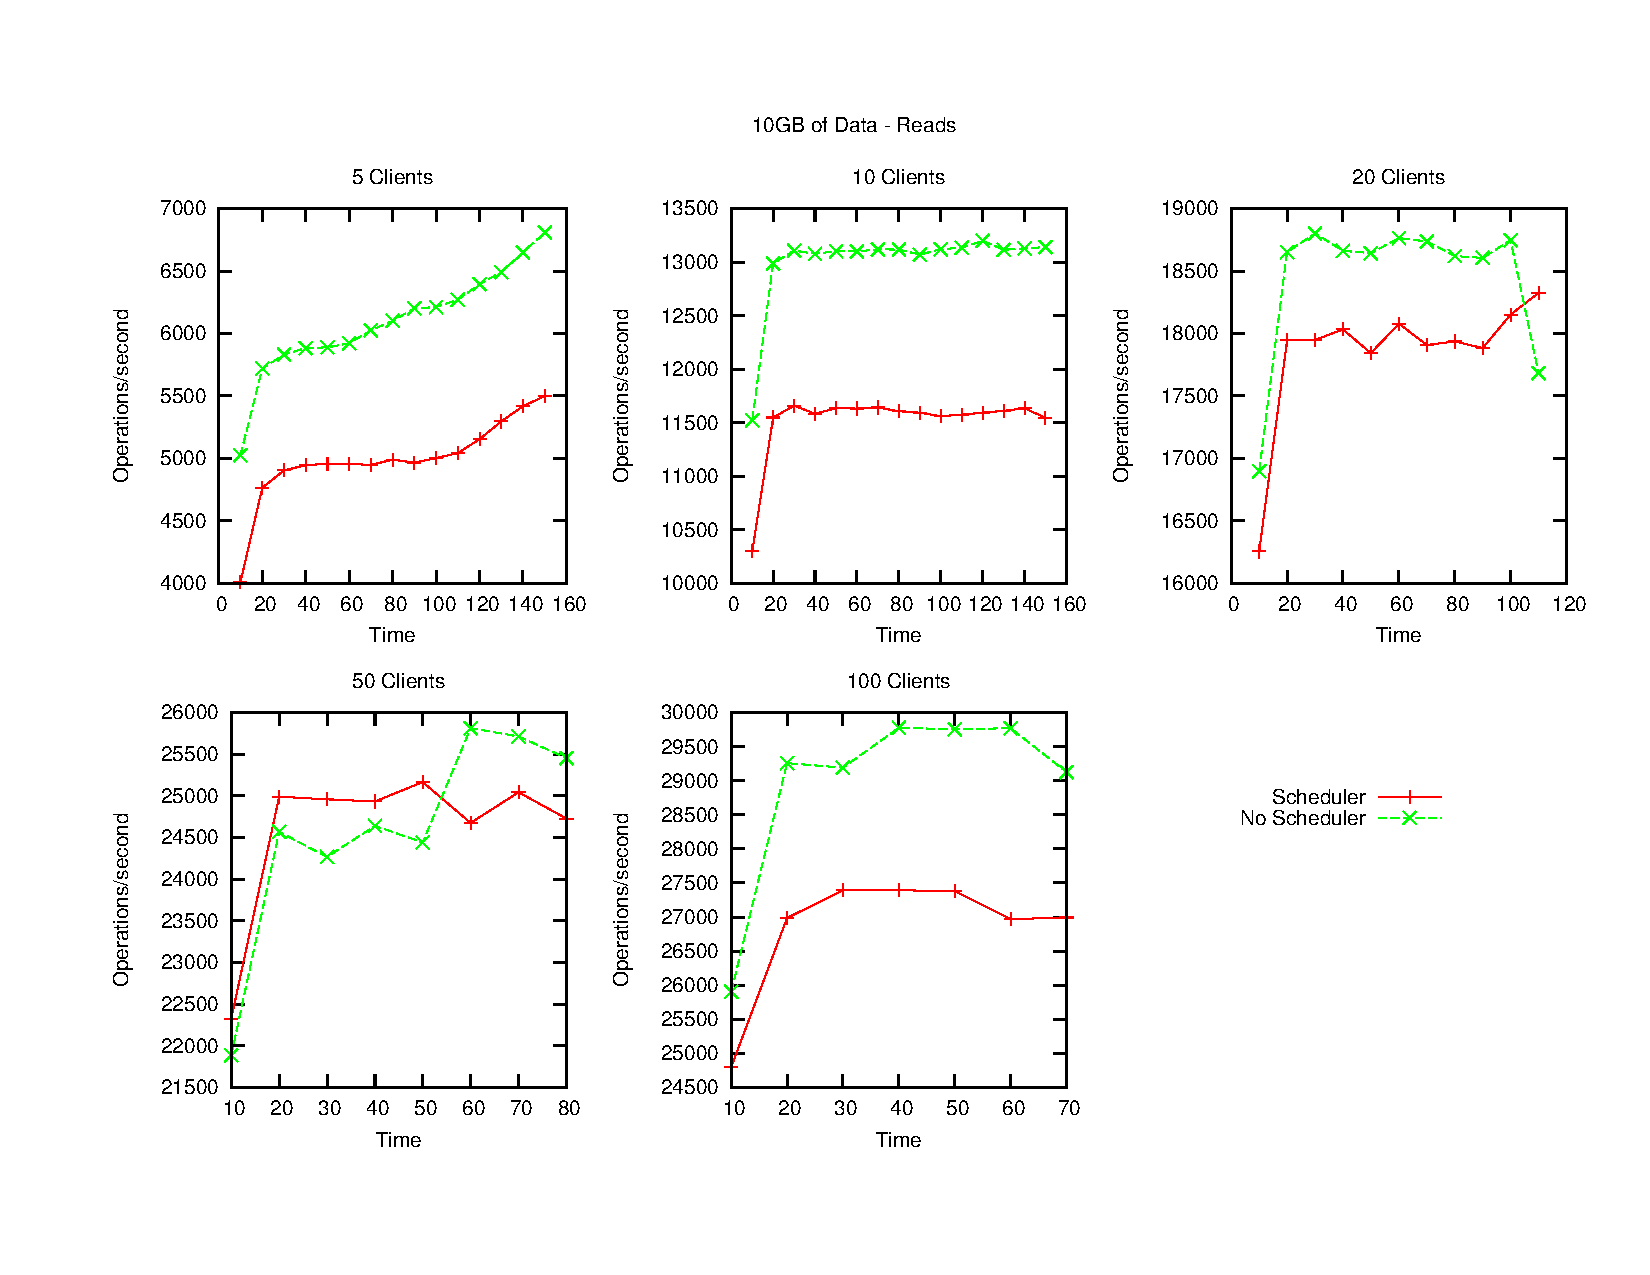
\includegraphics[scale=0.63]{images/10GB_Reads.pdf}
\vspace{-15pt}
\caption{The experimental results of performing the 100\% read workload on the 10GB database.}
\label{fig:10g_reads}
\end{figure*}

The results of the 10GB experiment are shown in Figure~\ref{fig:10g_reads}. As can be seen, the version of Cassandra using the resource based query assignment did not perform as well as the baseline Cassandra in any of the five experiments. However, the difference in throughput between the scheduled and baseline versions tended to stay constant throughout the course of each experiment. As well, the ratio of the difference between experiments was very similar. This seems to indicate that the overhead of performing the additional assignment logic is what resulted in the decrease in performance. We also monitored the servers resource usage during the course of the experiment and found that the server was never heavily loaded, which means that the performance difference is very minor (i.e., there is no noticable difference between 10\% CPU usage and 12\% CPU usage).

\begin{figure*}[t]
\centering
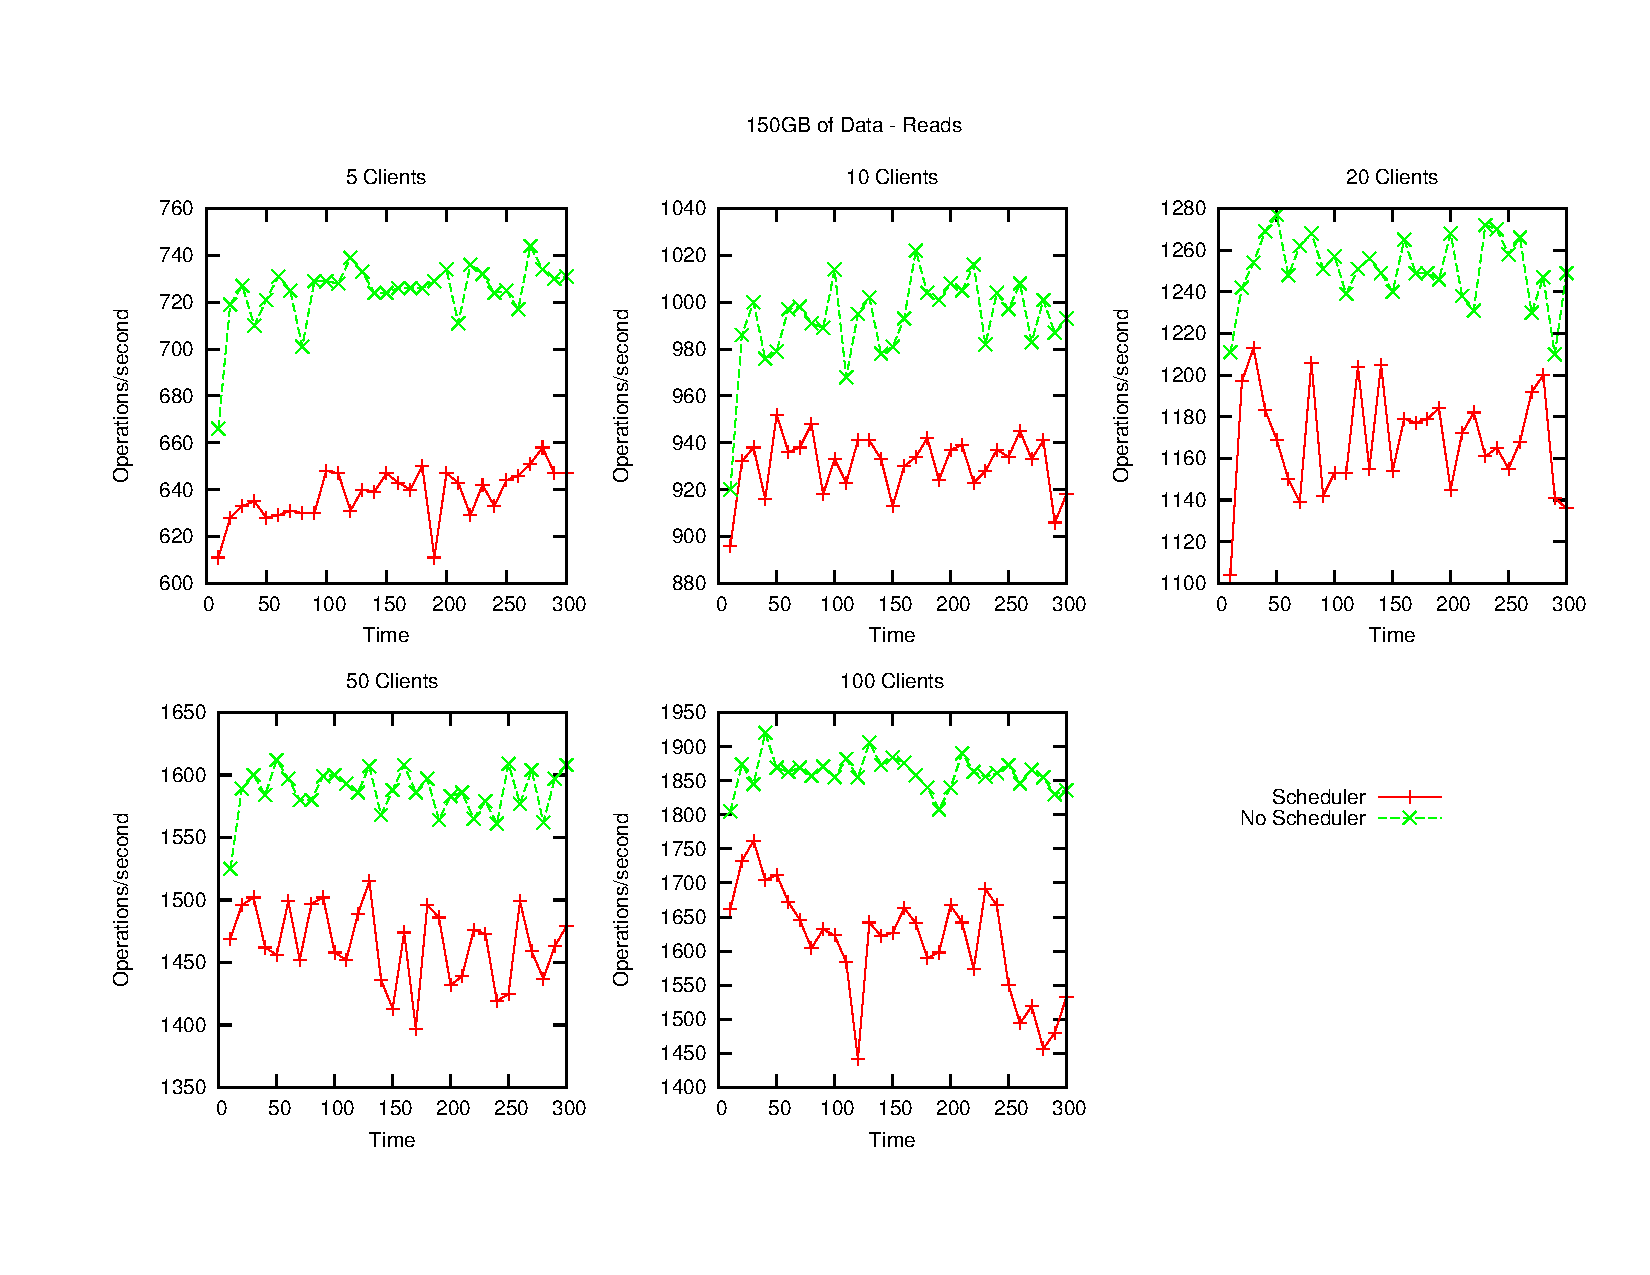
\includegraphics[scale=0.63]{images/150GB_Reads.pdf}
\vspace{-15pt}
\caption{The experimental results of performing the 100\% read workload on the 150GB database.}
\label{fig:150g_reads}
\end{figure*}

The results of the 150GB experiment are shown in Figure~\ref{fig:150g_reads}. Even with 100 parallel clients sending queries to the database, the node servers CPU usage and memory usage was still quite low. It seems that hard-disk accesses are the major bottleneck, which we have not accounted for in our method. The Cassandra read-digest~\cite{http://wiki.apache.org/cassandra/DigestQueries} also accounts for the slow performance, as even though you may read the data from the lowest resource usage server, you still need to access the other two servers in order to get the hash value and timestamp for the data.

The introduced overhead of managing the hash table also seems to be at least partially responsible for the poor performance. In the baseline version, Cassandra does try to access the list of endpoints, and only sends the query to the first endpoint. In our version, we are not only traversing the list of valid replicas, but also swapping entries in that list (to sort it by resource usage). We are also storing the resource usage values in a Java HashMap, which starts to perform poorly when many threads are accessing it at one time (this is apparent from the extremely poor performance of the 100 client experiment).

Because of the read digest, you still need to go to the poor performing servers to get a hash value. Running the experiment using scans shows that this is not always the case.


\begin{figure*}[t]
\centering
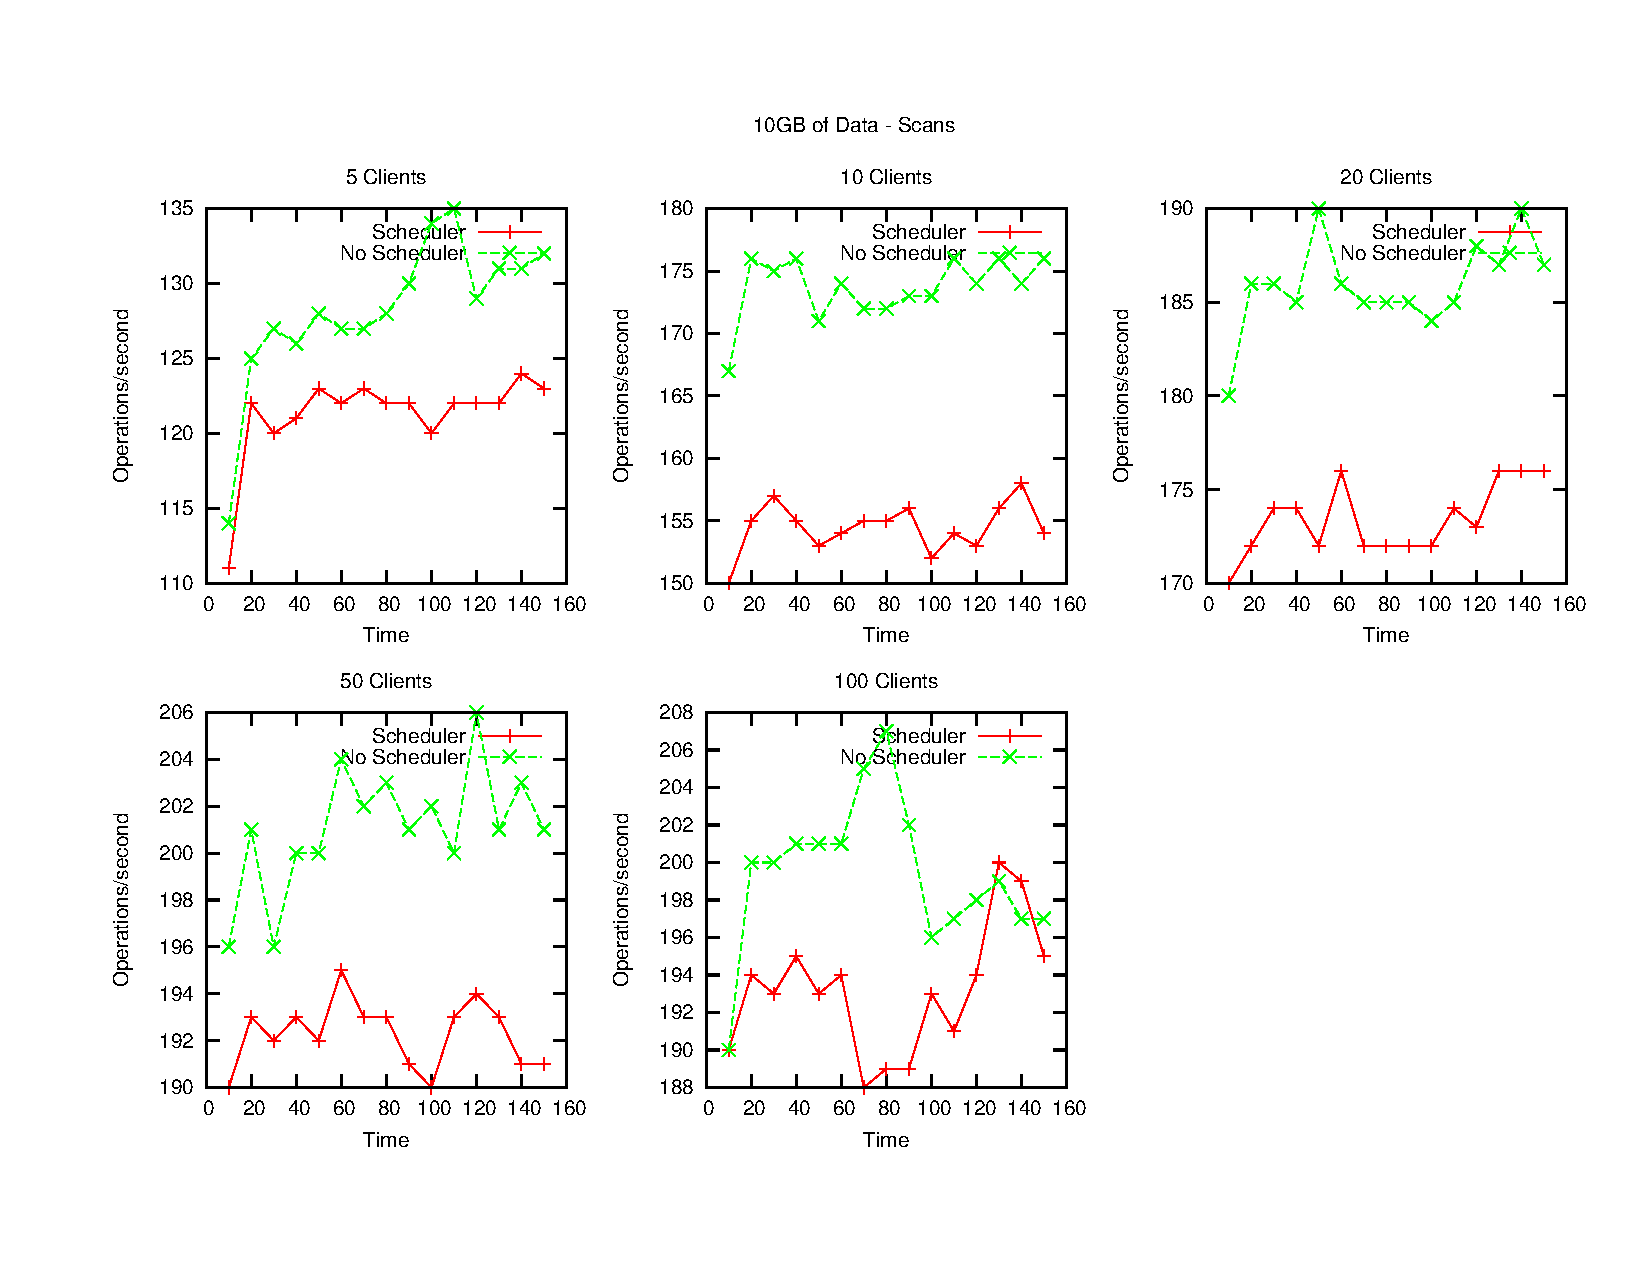
\includegraphics[scale=0.63]{images/10GB_Scans.pdf}
\vspace{-15pt}
\caption{The experimental results of performing the 100\% scan workload on the 10GB database.}
\label{fig:10g_scans}
\end{figure*}

We only ran the scan workload with 10GB of data. As the performance of the scheduler when performing scans was no better than the performance without then it is clear that the scans do not work. The primary difference between scans and reads is that the scan does not perform a read digest, thus removing the need to call every server to retrieve the value for a single key.

The results of the 10GB experiment are shown in Figure~\ref{fig:10g_scans}.

\begin{figure*}[t]
\centering
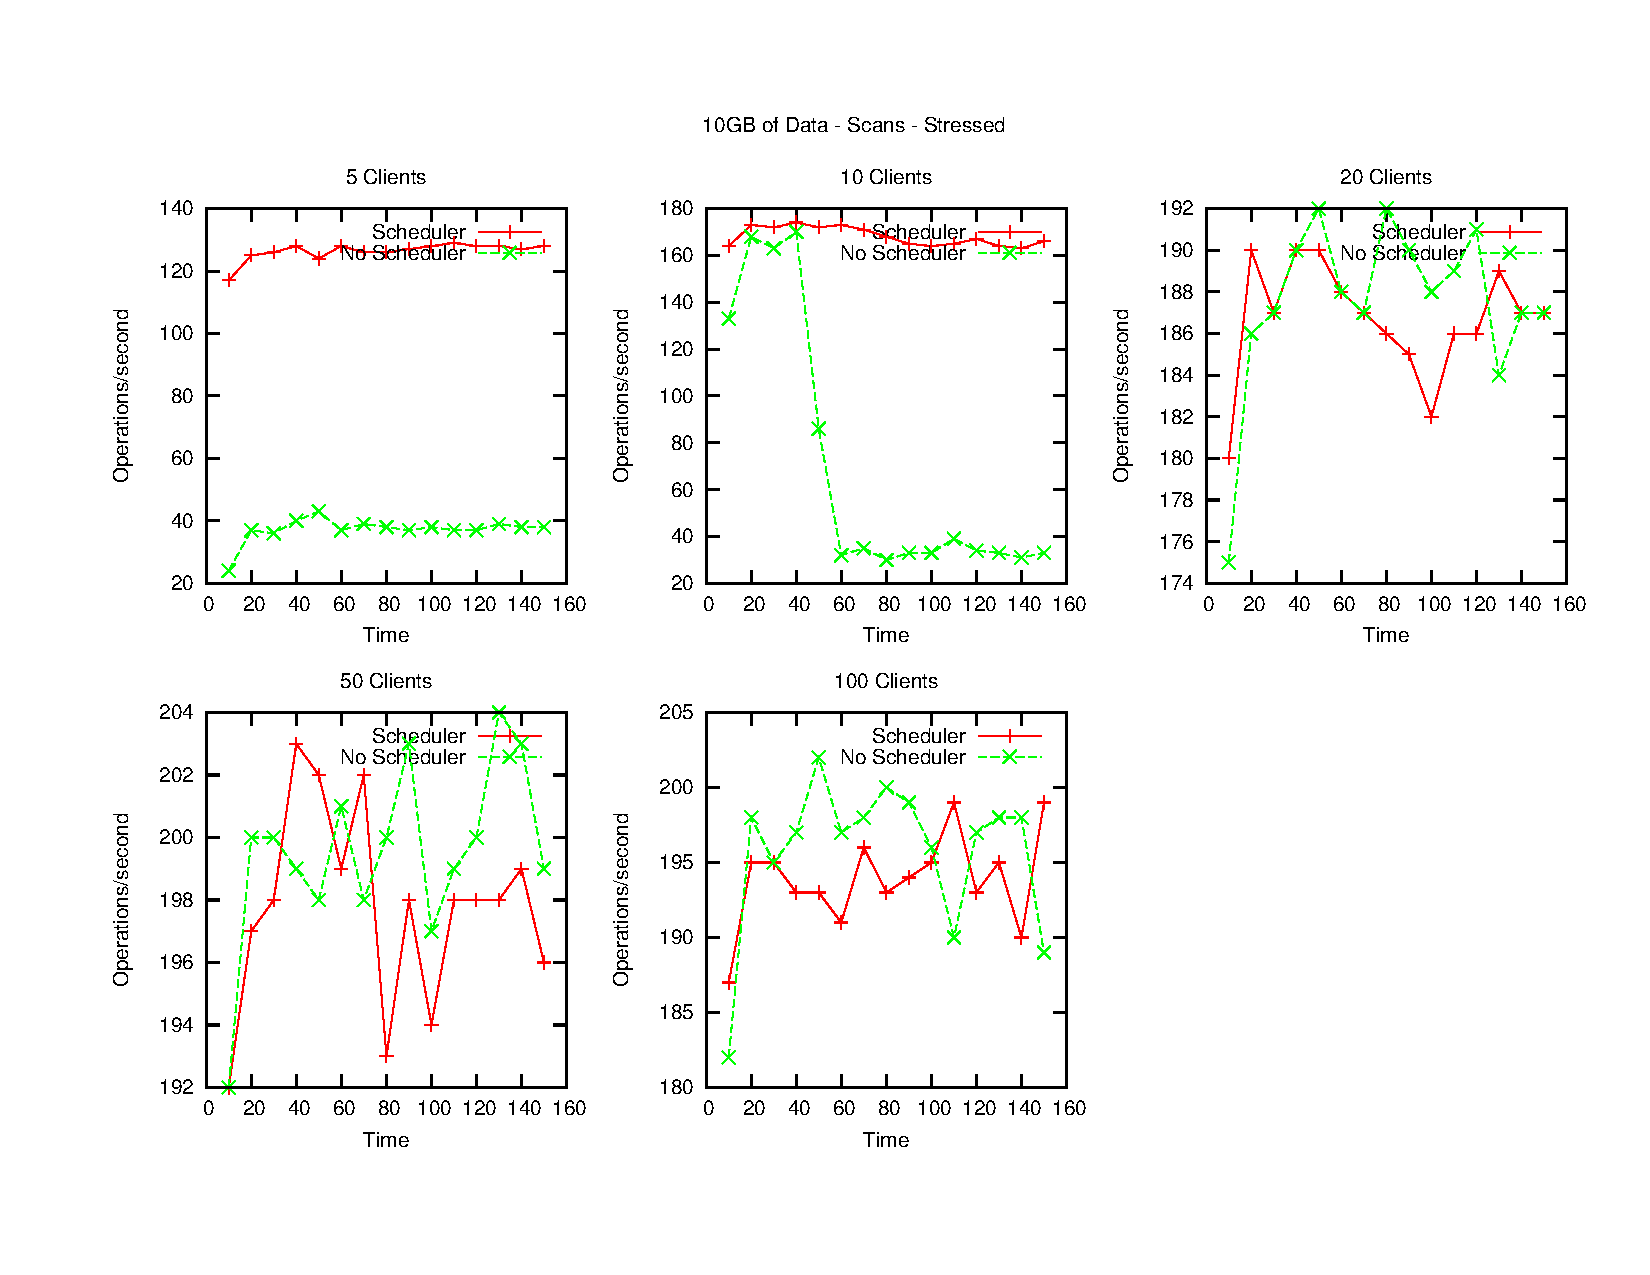
\includegraphics[scale=0.63]{images/10GB_Scans_Stressed.pdf}
\vspace{-15pt}
\caption{The experimental results of performing the 100\% scan workload on the 10GB database (where every second node is stressed).}
\label{fig:10g_scans_stressed}
\end{figure*}

We also ran the scans workload while introducing artificial workload into the server. This is a fairly contrived case, but is the ideal case for our work. The results of the 5 and 10 client experiments are shown in Figure~\ref{fig:10g_scans_stressed}. In these cases you can see that the resource aware assignment has much better performance than the baseline Cassandra. This is because the resource aware assignment will consider that every second server is overloaded. The figures for the cases with 20, 50 and 100 clients are not shown because performing experiment on the baseline version of Cassandra resulted in the Cassandra code continually crashing.

\section{Discussion}
\todo{Need to fill in this with a small intro sentence}

\subsection{Re-examining the Resource Usage formula}
As can be seen, our approach yields a small improvement to the baseline Cassandra performance. However, this improvement is not nearly as good as we had hoped. Our intuition is that the performance is gains are minimal because the formula that we have used to calculate the resource usage score does not totally suit our purpose~\cite{Gray and Black Box}. To confirm this intuition we performed an experiment that compared the resource usage to the query execution time in a Cassandra instance. 

The setup for the resource usage experiments is different than the setup for the primary experiments. This experiment was performed on a single Cassandra instance on a single machine with a 4-core 2.6Ghz processor and 8GB of memory. The server also contained a solid-state drive instead of the hard disk drive used in the servers in the cluster. The settings for YCSB and Cassandra were identical, except that the replication factor was set to one.

The CPU usage and memory usage was recorded every 250ms, and the query execution time was recorded for each query. The queries that executed in that 250ms window had their execution time averaged. The CPU usage and memory usage were used to calculate the resource usage of the server for each 250ms interval. The results were gathered over a 300 second interval using 10 parallel YCSB clients. We do not believe that the results would be significantly different for other numbers of parallel YCSB clients, but we have not confirmed this.

The results from the experiment are shown in Figure A. There appears to be little correlation between the resource usage score and the query execution time. When the resource usage score is higher, there are slightly more outliers that require a longer execution time, but in most cases the execution time seems to be independent of the resource usage. In addition, the resource usage scores tend to either be very low or very high. While this experiment was running, we were also attempting to artificially load the server. However, this seemed to make little difference to the resource usage score. 

This experiment seems to indicate that the current formula is not ideal for determining the resource usage of the server. However, we believe that this could still work if the formula was changed to reflect how some variables affect the query execution time much more.  Additional variables can also be added that affect query execution time. For example, one of the primary bottlenecks in any database system is the hard disk, and we do not consider any variables related to the disk (e.g., disk access throughput).

Something to note is that the heap memory of the Cassandra instance rarely exceeded 1GB. Meaning that the memory usage score had little effect during the normal experiments. Even when the server was being artificially loaded the heap memory therefore has little effect. This also means that little data is being cached, which increases the importance of measuring the disk load.

\section{Future Work}

\section{Conclusion}

\bibliographystyle{abbrv}
\bibliography{refs}

\end{document}